\documentclass[11pt, a4paper]{article}
\usepackage{pdfpages}
\usepackage{parallel}
\usepackage[T2A]{fontenc}
\usepackage{ucs}
\usepackage[utf8x]{inputenc}
\usepackage[polish,english,russian]{babel}
\usepackage{hyperref}
\usepackage{rotating}
\usepackage[inner=2cm,top=1.8cm,outer=2cm,bottom=2.3cm,nohead]{geometry}
\usepackage{listings}
\usepackage{graphicx}
\usepackage{wrapfig}
\usepackage{longtable}
\usepackage{indentfirst}
\usepackage{array}
\usepackage{tikzsymbols}
\usepackage{soul}
\usepackage[ruled,vlined]{algorithm2e}
%\counterwithout{figure}{section} 

\usepackage{url}
\makeatletter
\g@addto@macro{\UrlBreaks}{\UrlOrds}
\makeatother

\newcolumntype{P}[1]{>{\raggedright\arraybackslash}p{#1}}
\frenchspacing
\usepackage{fixltx2e} %text sub- and superscripts
\usepackage{icomma} % коскі ў матэматычным рэжыме
\PreloadUnicodePage{4}

\newcommand{\longpage}{\enlargethispage{\baselineskip}}
\newcommand{\shortpage}{\enlargethispage{-\baselineskip}}

\def\switchlang#1{\expandafter\csname switchlang#1\endcsname}
\def\switchlangbe{
\let\saverefname=\refname%
\def\refname{Літаратура}%
\def\figurename{Іл.}%
}
\def\switchlangen{
\let\saverefname=\refname%
\def\refname{References}%
\def\figurename{Fig.}%
}
\def\switchlangru{
\let\saverefname=\refname%
\let\savefigurename=\figurename%
\def\refname{Литература}%
\def\figurename{Рис.}%
}

\hyphenation{admi-ni-stra-tive}
\hyphenation{ex-pe-ri-ence}
\hyphenation{fle-xi-bi-li-ty}
\hyphenation{Py-thon}
\hyphenation{ma-the-ma-ti-cal}
\hyphenation{re-ported}
\hyphenation{imp-le-menta-tions}
\hyphenation{pro-vides}
\hyphenation{en-gi-neering}
\hyphenation{com-pa-ti-bi-li-ty}
\hyphenation{im-pos-sible}
\hyphenation{desk-top}
\hyphenation{elec-tro-nic}
\hyphenation{com-pa-ny}
\hyphenation{de-ve-lop-ment}
\hyphenation{de-ve-loping}
\hyphenation{de-ve-lop}
\hyphenation{da-ta-ba-se}
\hyphenation{plat-forms}
\hyphenation{or-ga-ni-za-tion}
\hyphenation{pro-gramming}
\hyphenation{in-stru-ments}
\hyphenation{Li-nux}
\hyphenation{sour-ce}
\hyphenation{en-vi-ron-ment}
\hyphenation{Te-le-pathy}
\hyphenation{Li-nux-ov-ka}
\hyphenation{Open-BSD}
\hyphenation{Free-BSD}
\hyphenation{men-ti-on-ed}
\hyphenation{app-li-ca-tion}

\def\progref!#1!{\texttt{#1}}
\renewcommand{\arraystretch}{2} %Іначай формулы ў матрыцы зліпаюцца з лініямі
\usepackage{array}

\def\interview #1 (#2), #3, #4, #5\par{

\section[#1, #3, #4]{#1 -- #3, #4}
\def\qname{LVEE}
\def\aname{#1}
\def\q ##1\par{{\noindent \bf \qname: ##1 }\par}
\def\a{{\noindent \bf \aname: } \def\qname{L}\def\aname{#2}}
}

\def\interview* #1 (#2), #3, #4, #5\par{

\section*{#1\\{\small\rm #3, #4. #5}}
\ifx\ParallelWhichBox\undefined%
    \addcontentsline{toc}{section}{#1, #3, #4}%
\else%
\ifnum\ParallelWhichBox=0%
    \addcontentsline{toc}{section}{#1, #3, #4}%
\fi\fi%

\def\qname{LVEE}
\def\aname{#1}
\def\q ##1\par{{\noindent \bf \qname: ##1 }\par}
\def\a{{\noindent \bf \aname: } \def\qname{L}\def\aname{#2}}
}

\newcommand{\interviewfooter}[1]{
\vskip 1em
\noindent \textit{#1}
}

\switchlang{ru}
\begin{document}

\title{1997 "--- ITAC Systems evolution MOUSE-TRAK trackball}
\date{}
\maketitle
\selectlanguage{russian}
Трекбол evolution MOUSE-TRAK выпущен техасской компанией ITAC Systems, специализировавшейся в первую очередь на высококачественных эргономичных трекболах для профессионального применения.

Разработчик позиционировал себя как пионер в производстве трекболов для Unix-систем и X-терминалов, выпустив модель MOUSE-TRAK в конце восьмидесятых. Появившиеся как средство решения проблемы с возникавшим у ряда пользователей мыши туннельным синдромом запястий, трекболы MOUSE-TRAK сохраняли классический индустриальный дизайн до 1997 года, когда в дополнение к классическому MOUSE-TRAK была выпущена в продажу модель evolution с полностью переработанным корпусом \cite{announcement, description}.

\begin{figure}[h]
    \centering
    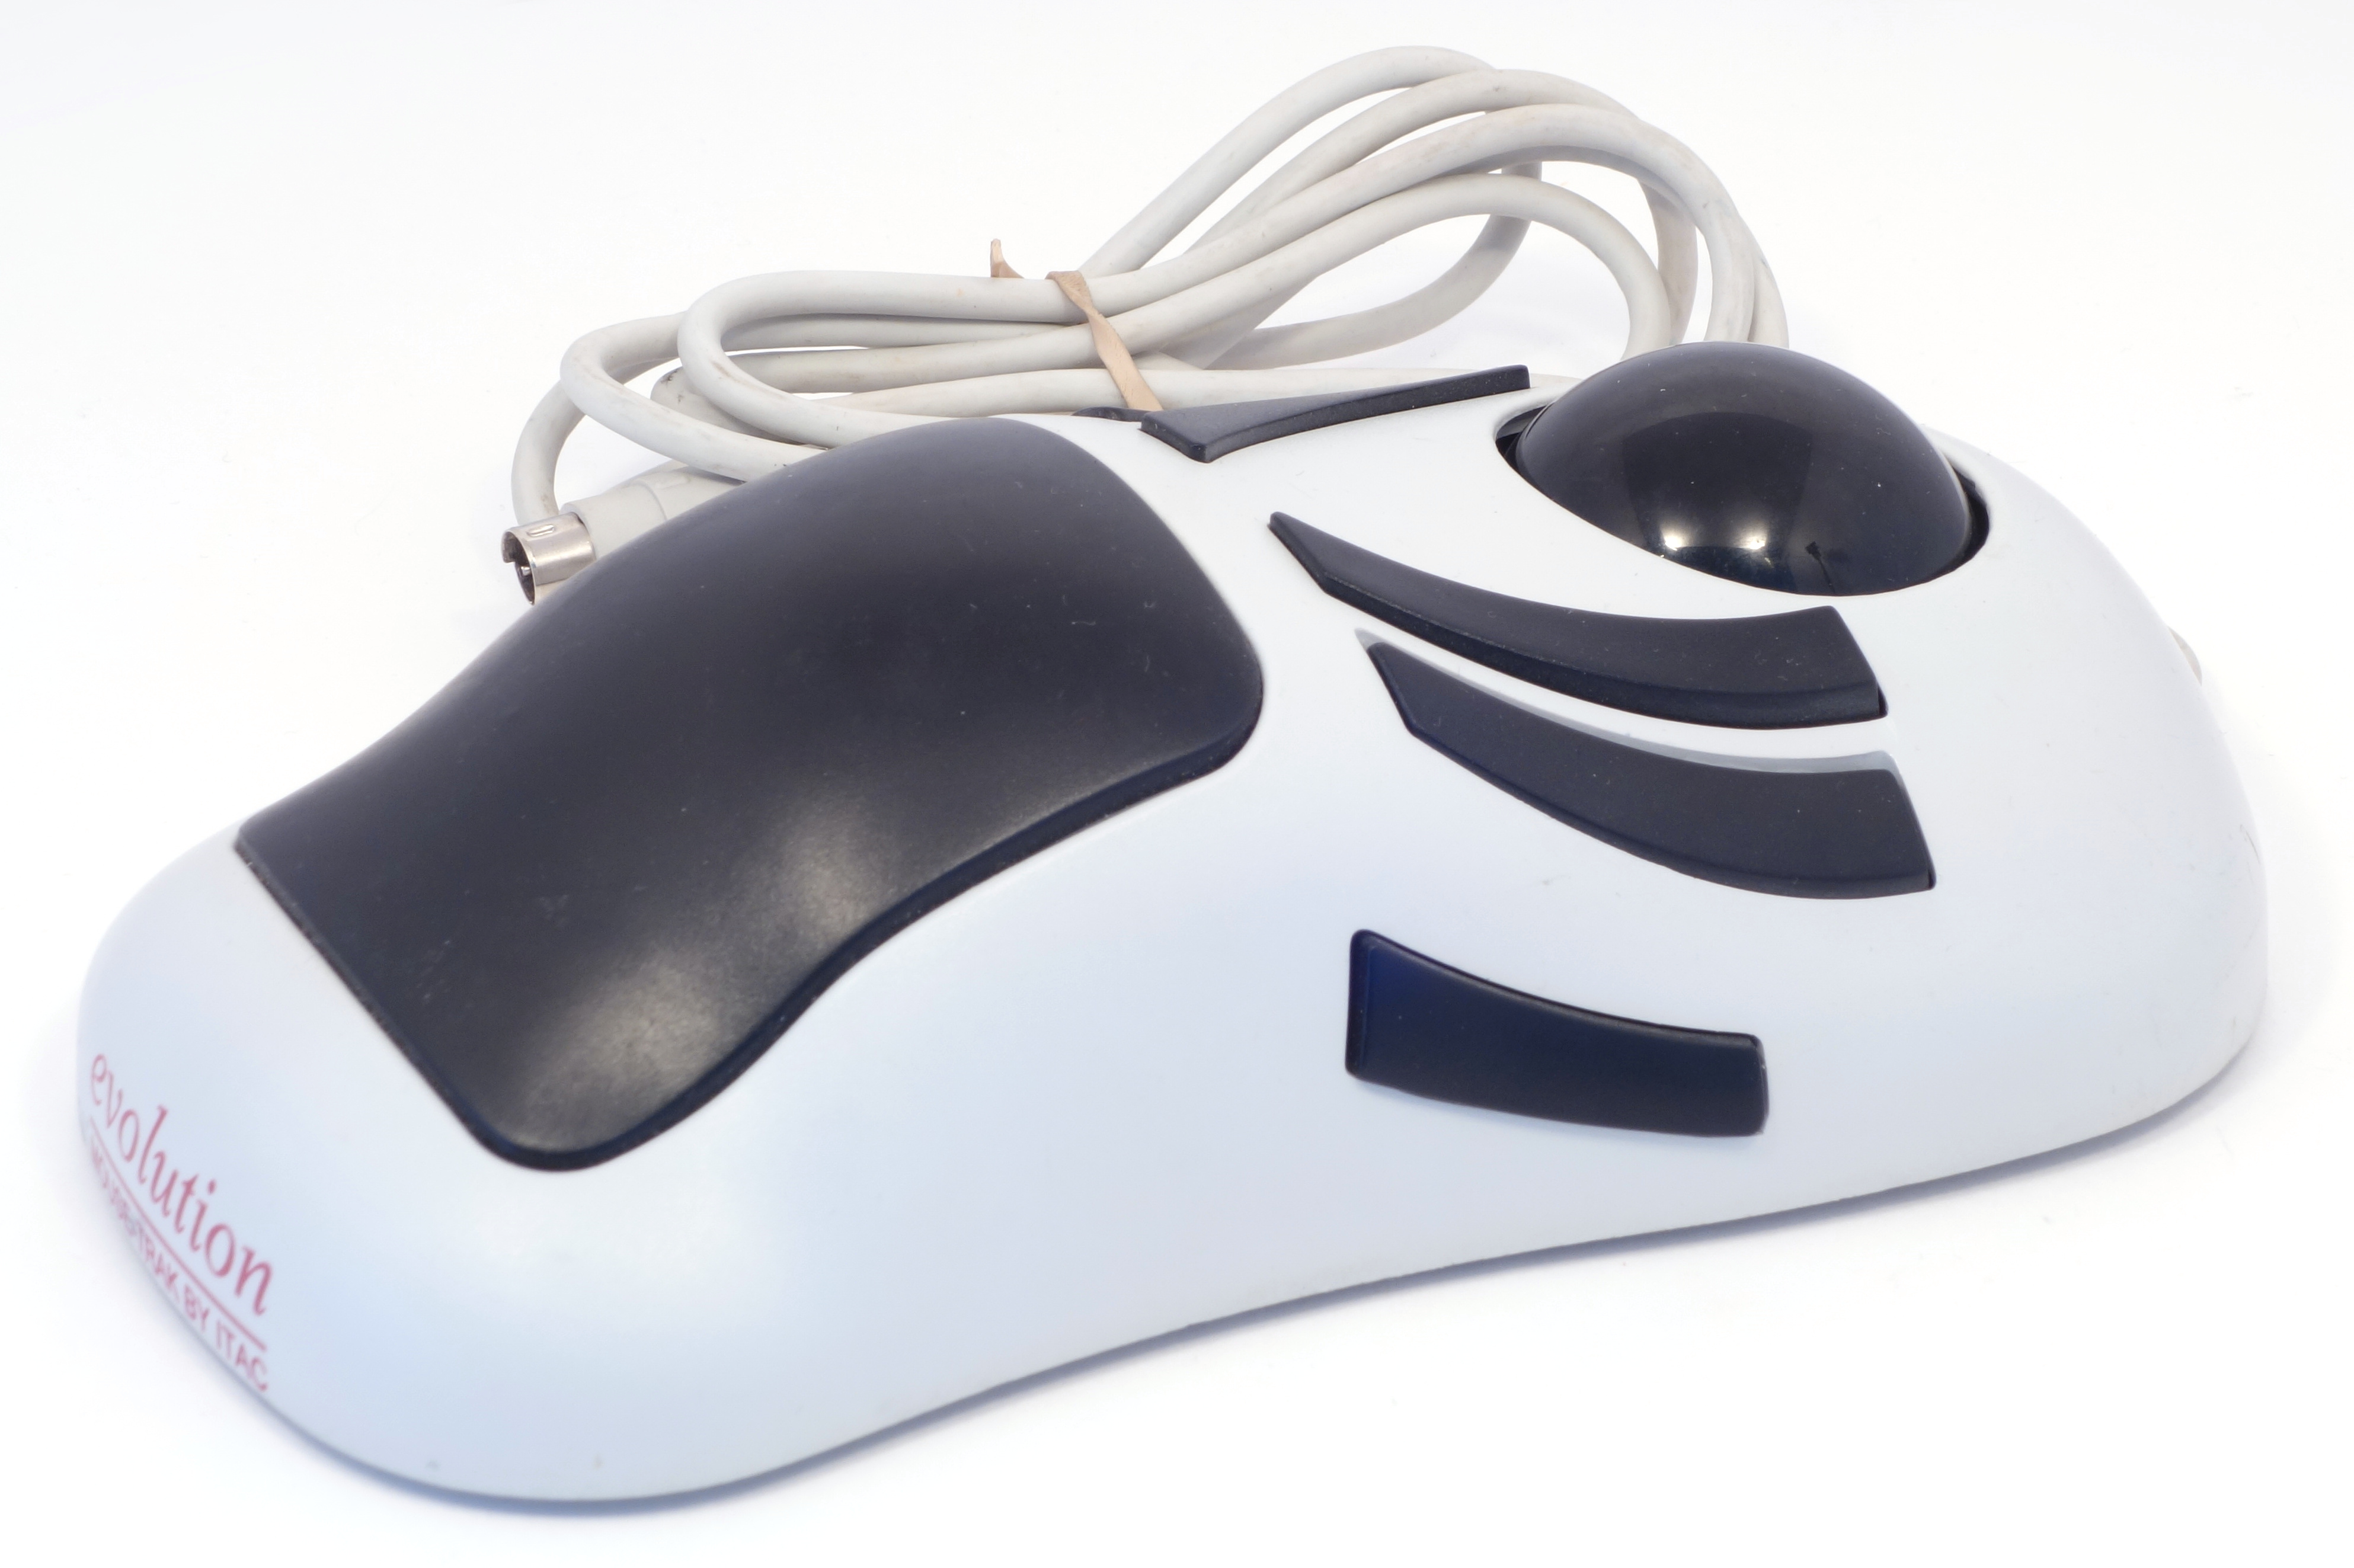
\includegraphics[scale=0.3]{1997_mousetrak_evolution/pic_30.jpg}
    \caption{Трекбол evolution MOUSE-TRAK}
    \label{fig:evolutionMOUSE-TRAK}
\end{figure}

На рис. \ref{fig:evolutionMOUSE-TRAKTopBottom} можно видеть верхнюю и нижнюю стороны трекбола.

\begin{figure}[h]
    \centering
    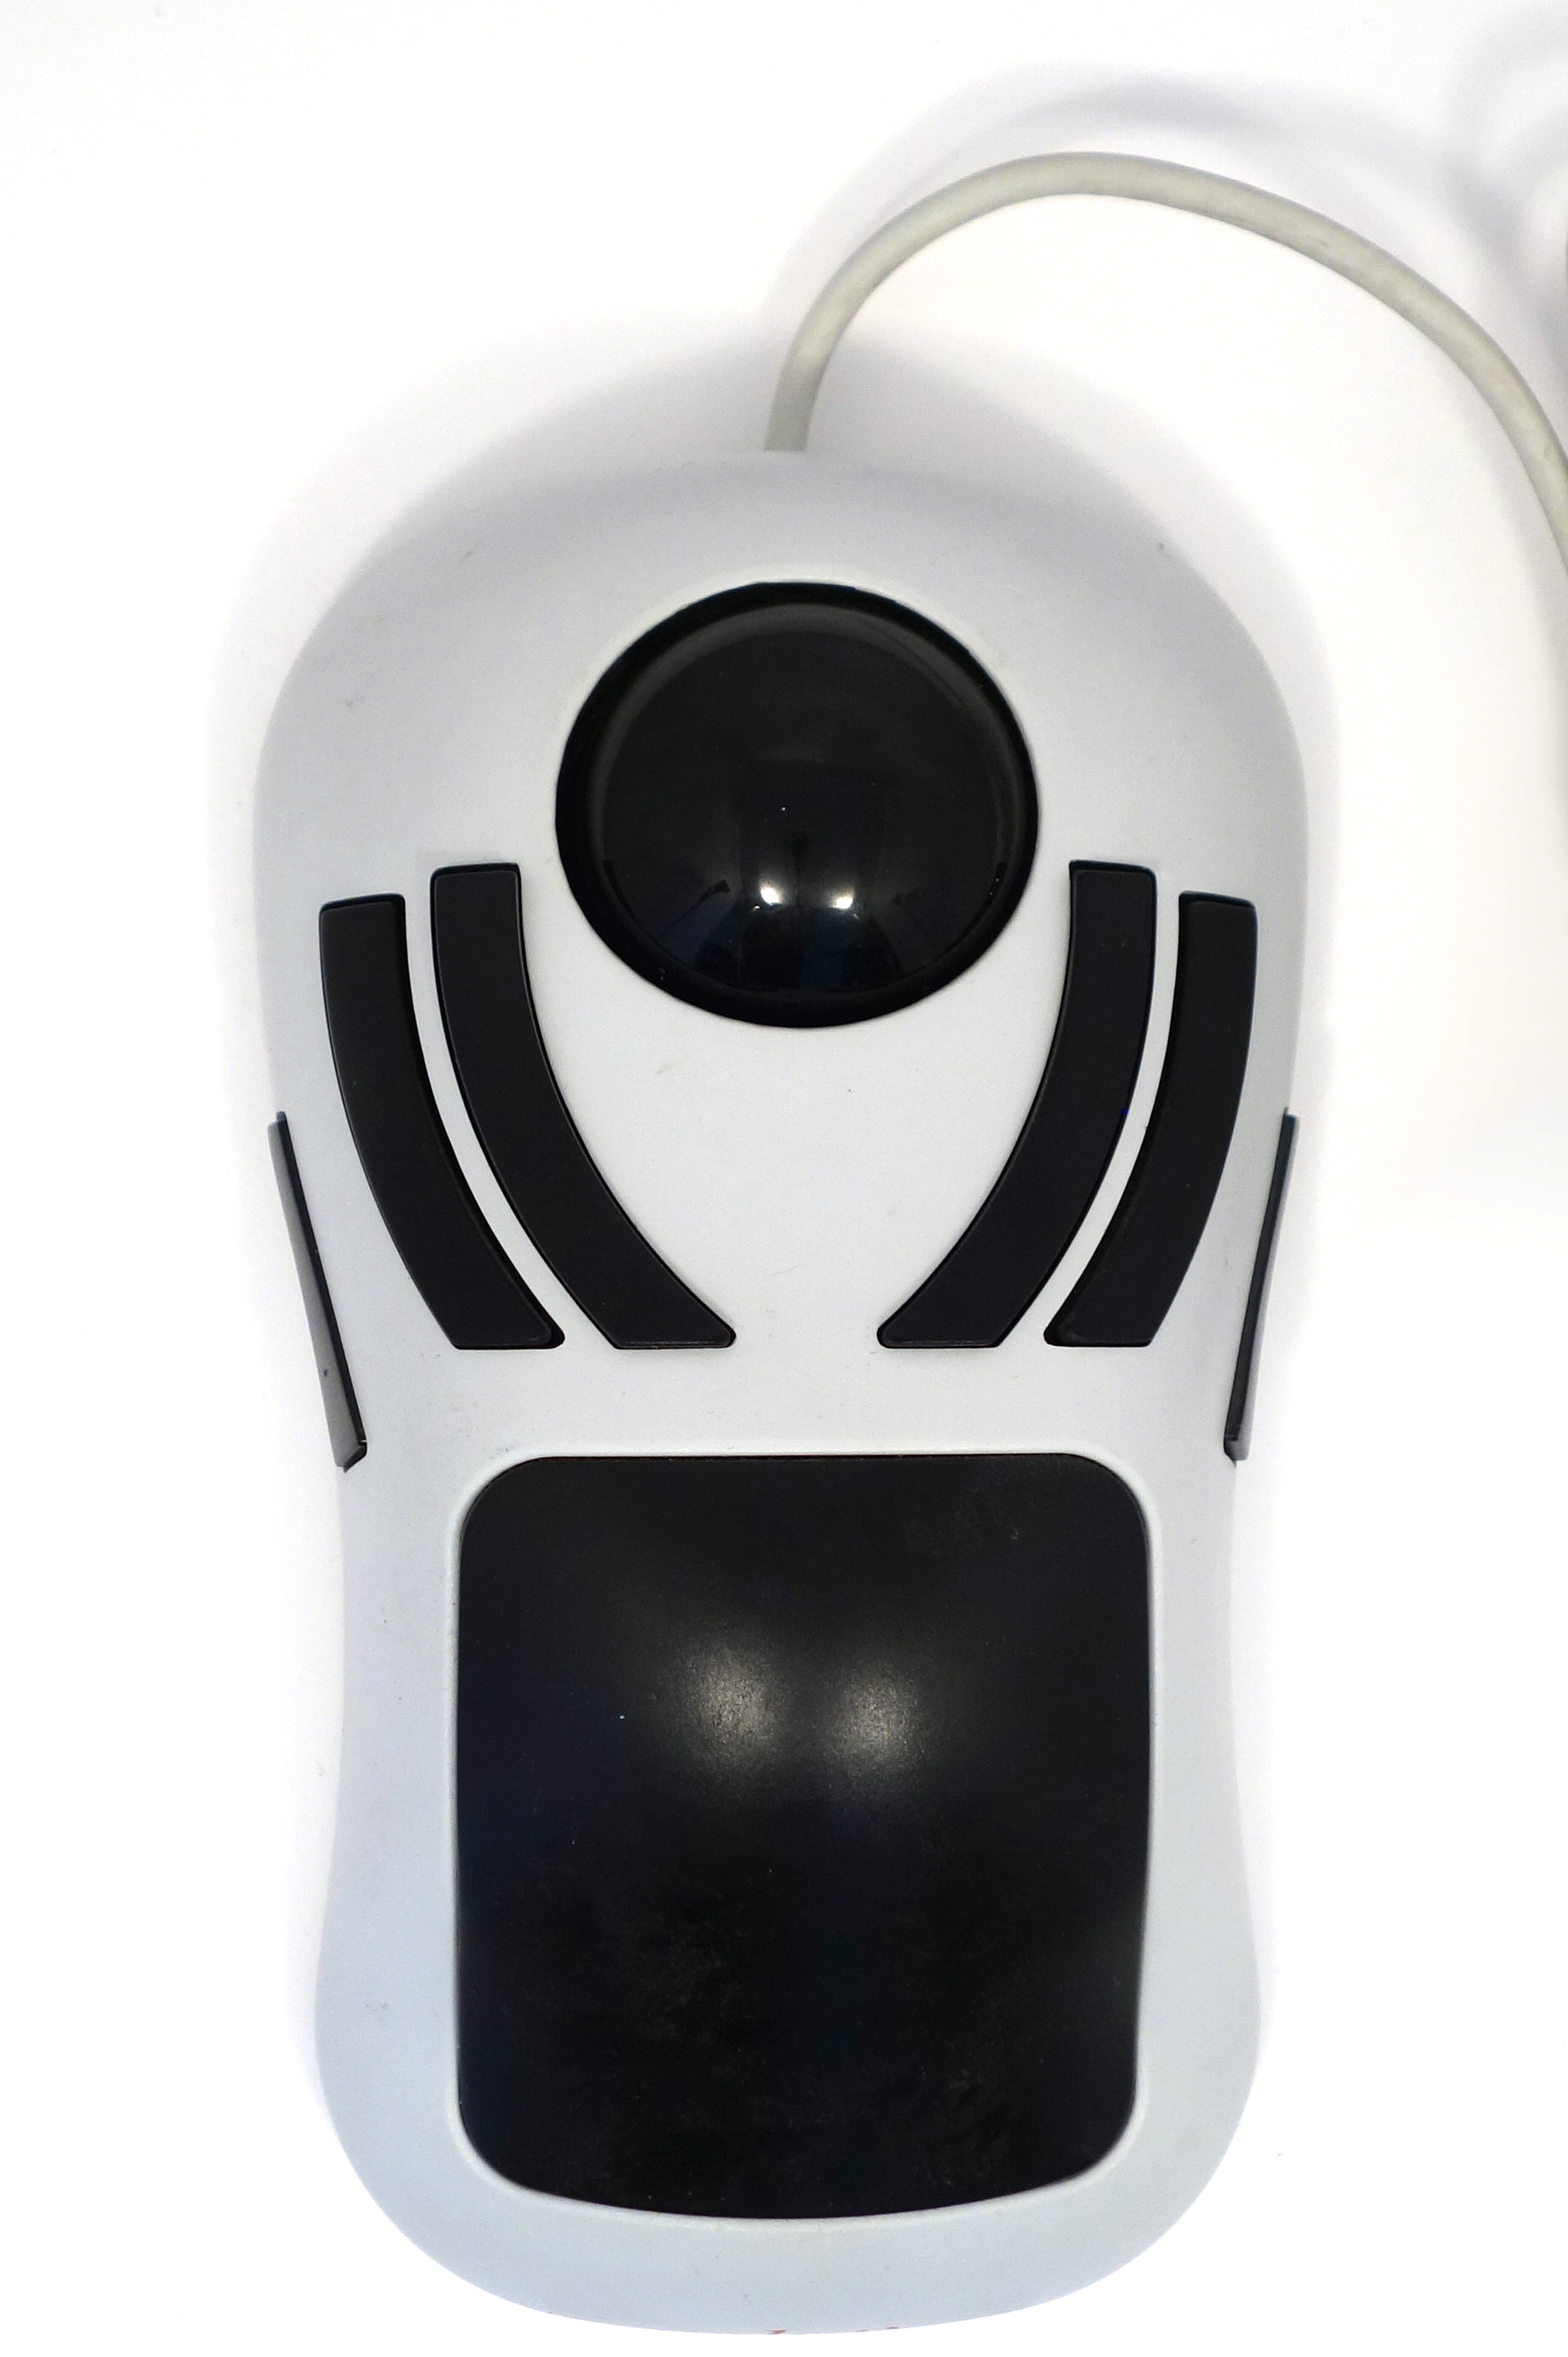
\includegraphics[scale=0.35]{1997_mousetrak_evolution/top_60.jpg}
    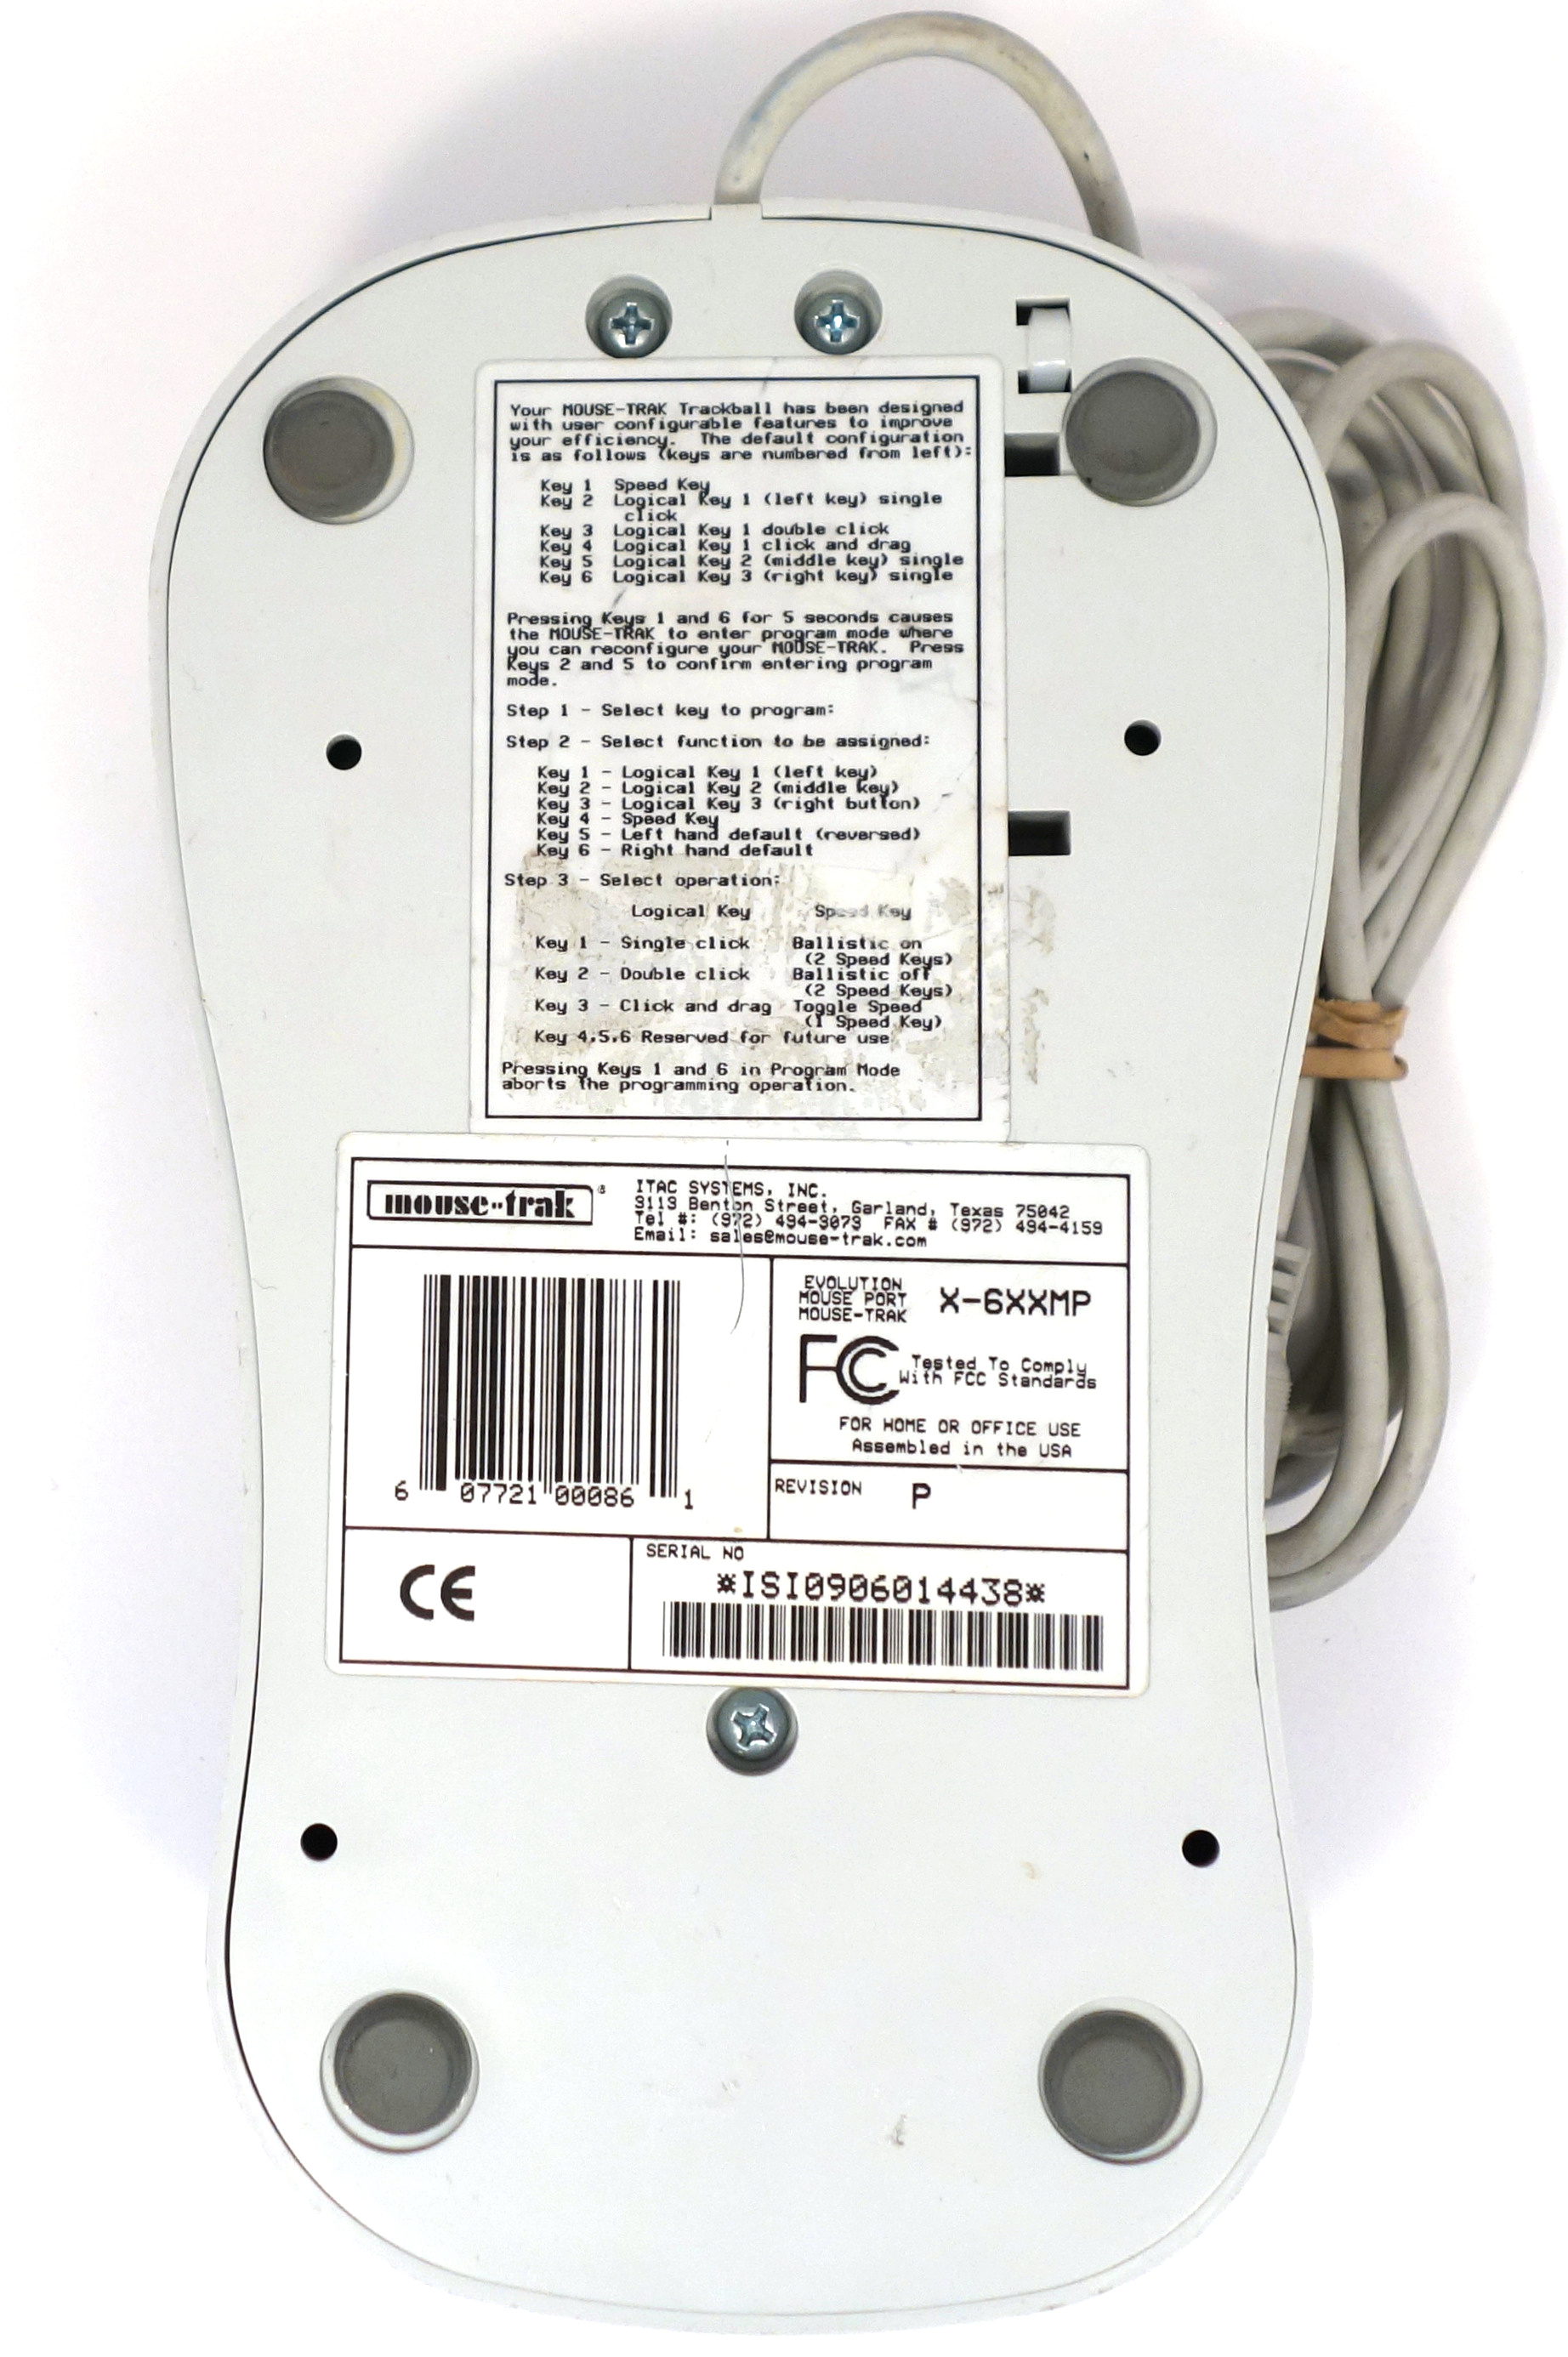
\includegraphics[scale=0.35]{1997_mousetrak_evolution/bottom_60.jpg}
    \caption{evolution MOUSE-TRAK, вид сверху и снизу}
     \label{fig:evolutionMOUSE-TRAKTopBottom}
\end{figure}

Корпус имеет белую матовую поверхность с контрастными черными элементами - шаром, шестью узкими длинными клавишами, расположенными <<зеброй>> перед шаром, и массивной мягкой опорой для руки, выполненной из ПВХ. На нижней части корпуса присутствуют резиновые ножки, обеспечивающие надежную фиксацию на поверхности стола, маркировка производителя и подробная инструкция по программированию клавиш трекбола.

Данное устройство является весьма габаритным (рис. \ref{fig:evolutionMOUSE-TRAKSize}). Иза сильно приподнятой опоры для руки, призванной снизить риск туннельного синдрома запястий, шар оказывается утопленным внутрь корпуса и визуально кажется меньшим, чем является в действительности.

\begin{figure}[h]
    \centering
    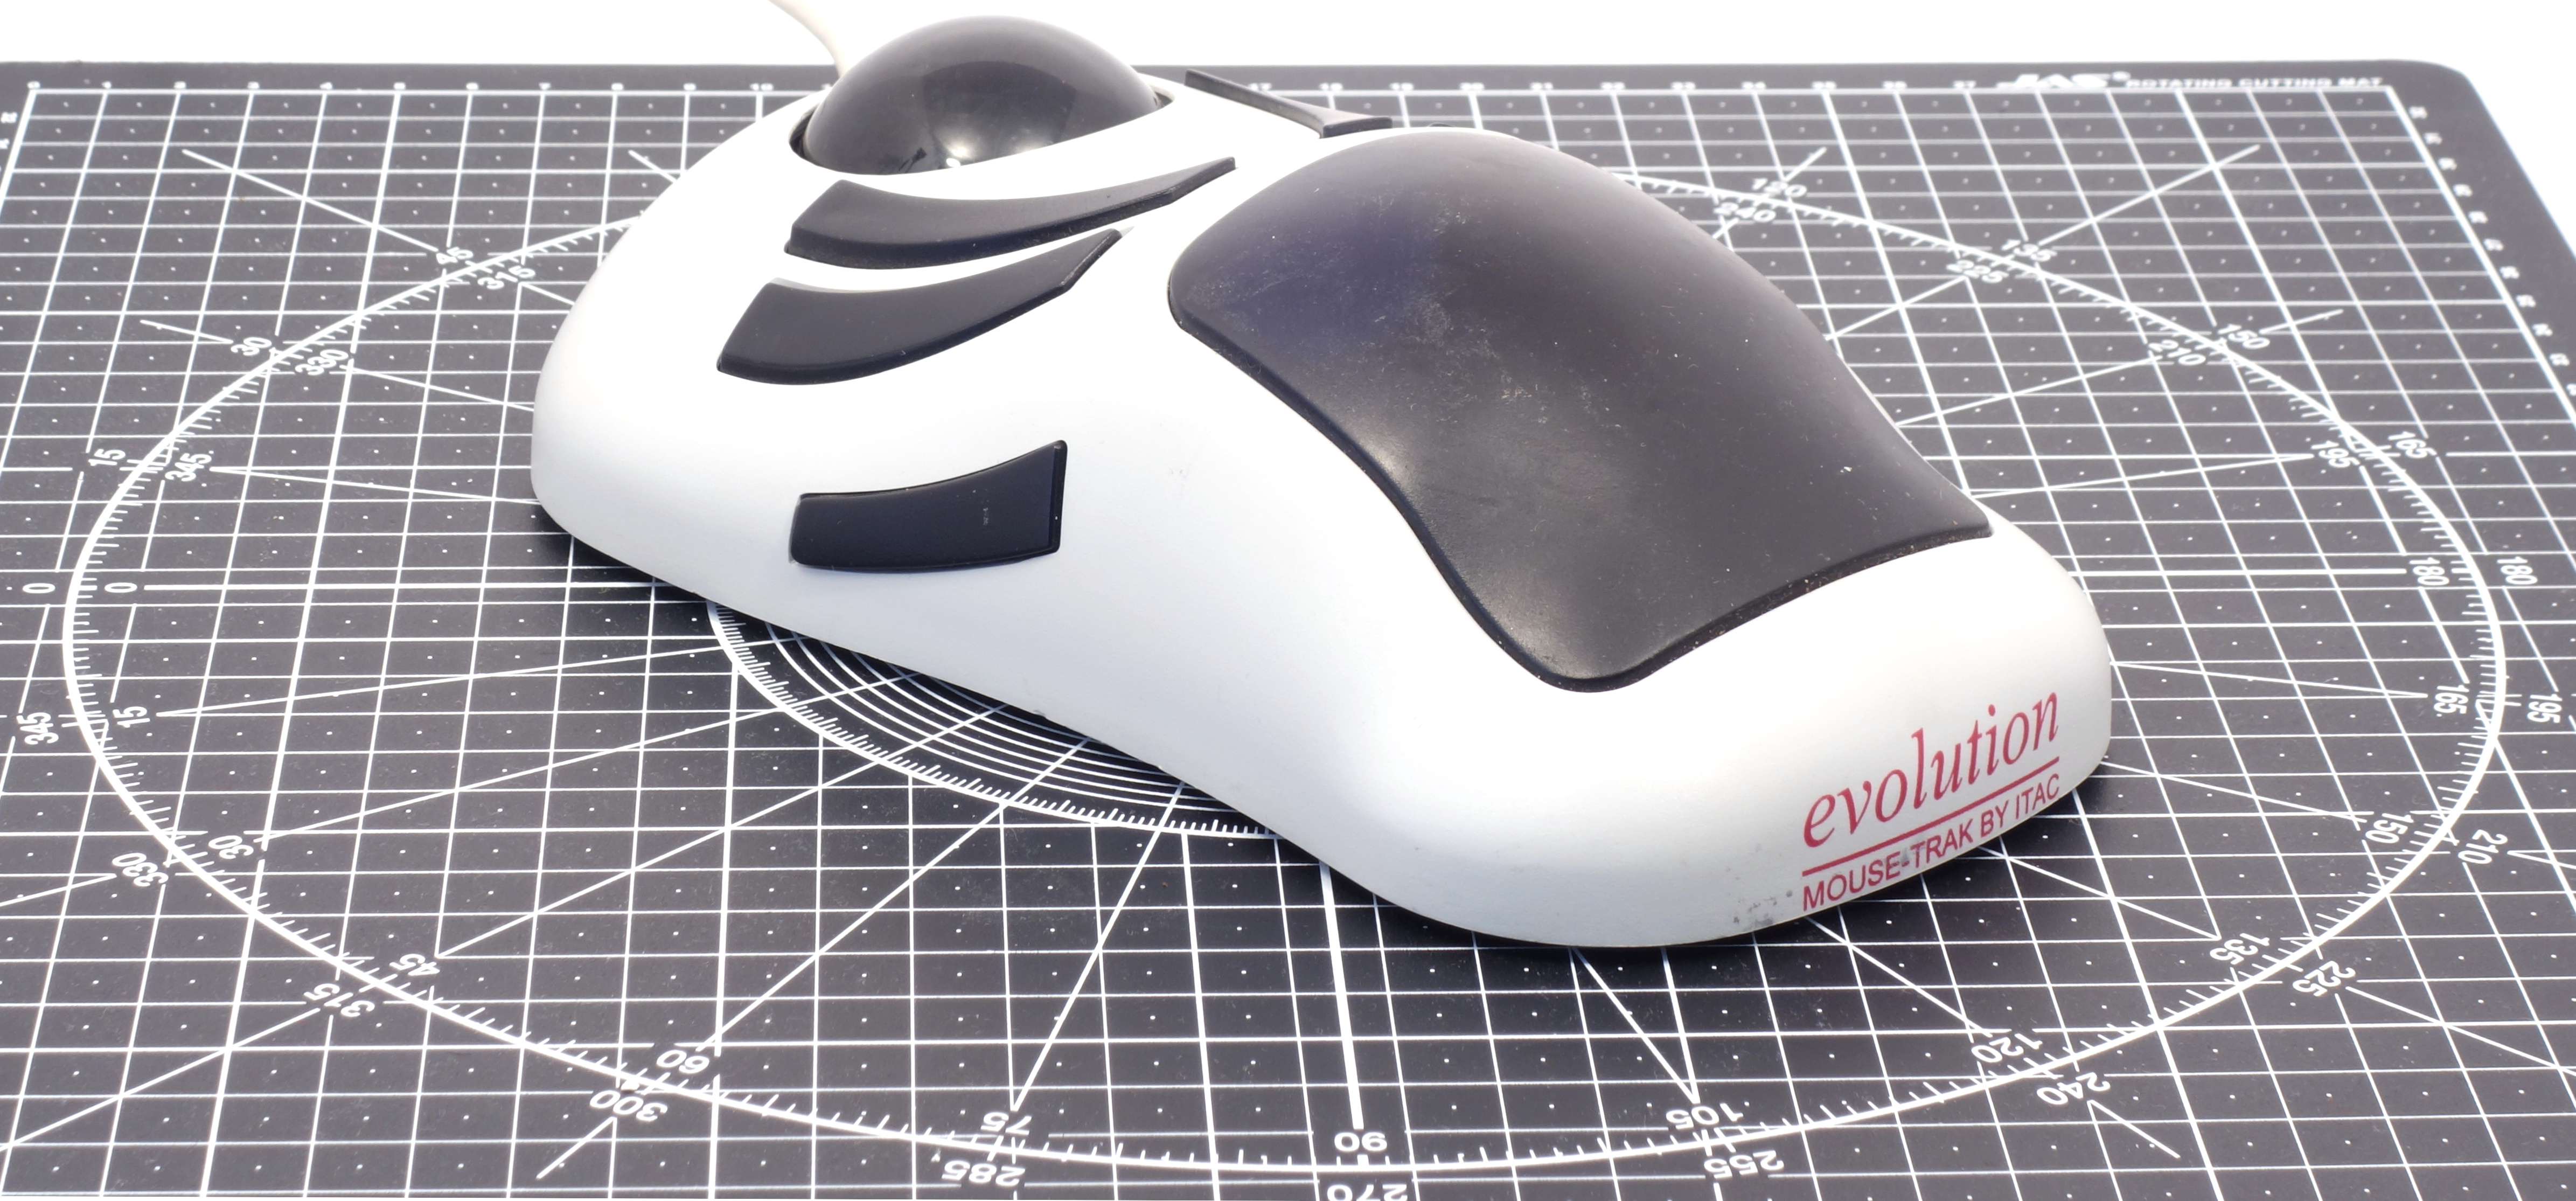
\includegraphics[scale=0.35]{1997_mousetrak_evolution/size_30.jpg}
    \caption{Изображение evolution MOUSE-TRAK на размерном коврике с шагом сетки 1~см}
    \label{fig:evolutionMOUSE-TRAKSize}
\end{figure}

Трекбол симметричен и одинаково удобен при использовании как правой так и левой рукой (особенно с учетом поддерживаемого им переназначения клавиш без использования драйвера).
Клавиши рассчитаны на нажатие большим пальцем и мизинцем \cite{pcmag}, в то время как остальные пальцы остаются свободными для позиционирования курсора (рис. \ref{fig:evolutionMOUSE-TRAKHand}). При этом по задумке разработчиков назначение наиболее часто используемых функций клавишам, находящимся вблизи шара, позволяет удобно использовать трекбол пользователям с меньшим размером кисти.

Режим перенастройки включается последовательным нажатием комбинаций клавиш, после чего, также путем последовательных нажатий, выполняется переназначение их функций (как уже упоминалось, детальная инструкция находится на нижней стороне корпуса).

Конфигурация клавиш по умолчанию выглядит следующим образом (слева направо): клавиша регулировки скорости, одинарный клик левой кнопкой мыши, двойной клик левой кнопкой мыши, клик левой кнопкой мыши с фиксацией (для перетаскивания), одинарный клик средней кнопкой мыши и одинарный клик правой кнопкой мыши \cite{advanced}.

Трекбол выпускался в двух модификациях, различавшихся интерфейсом (PS/2 и USB).

\begin{figure}[h]
    \centering
    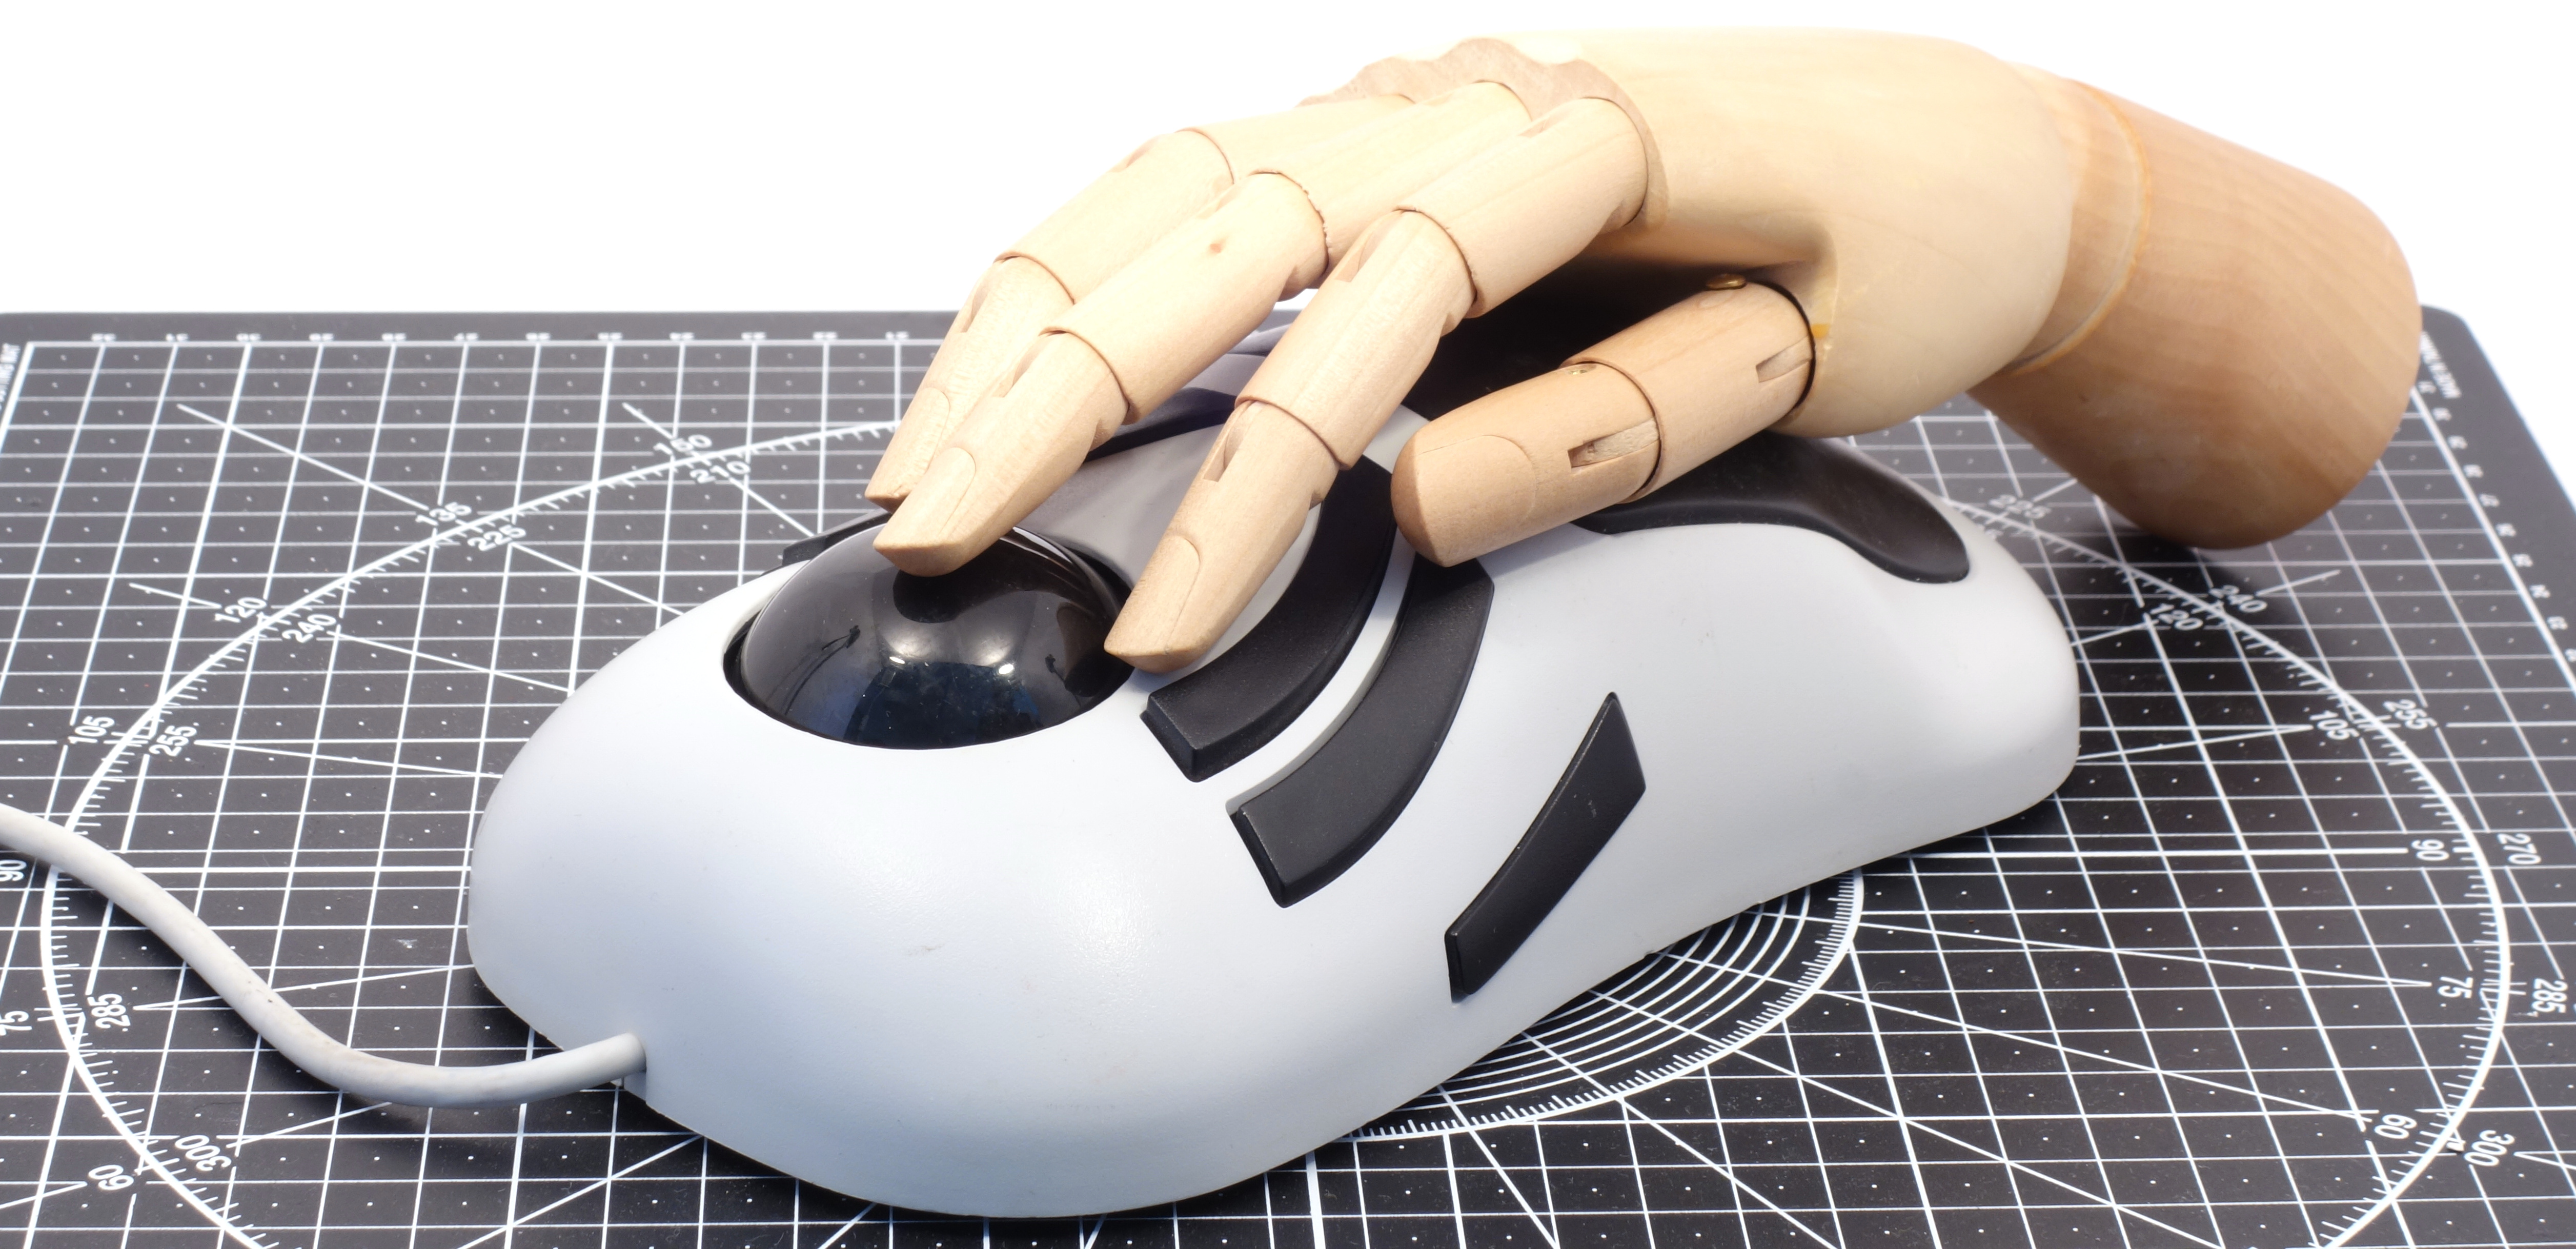
\includegraphics[scale=0.35]{1997_mousetrak_evolution/hand_30.jpg}
    \caption{evolution MOUSE-TRAK с моделью руки человека}
    \label{fig:evolutionMOUSE-TRAKHand}
\end{figure}

Внутреннее устройство трекбола показано на рис. \ref{fig:evolutionMOUSE-TRAKInside}. Как можно видеть, в нем используется классическая оптомеханическая схема. Ролики выполнены с использованием шарикоподшипников и металлических осей, что обеспечивает максимальную надежность и долговечность конструкции. На это делается упор и в описании производителя, где среди особенностей устройства подчеркивается использование подшипников и роликов из закаленной стали.

К недостаткам конструкции можно отнести отсутствие съемного кольца-защелки: учитывая, что большая часть шара скрыта внутри корпуса, его извлечение для чистки трекбола оказывается невозможным без разборки корпуса.

\begin{figure}[h]
    \centering
    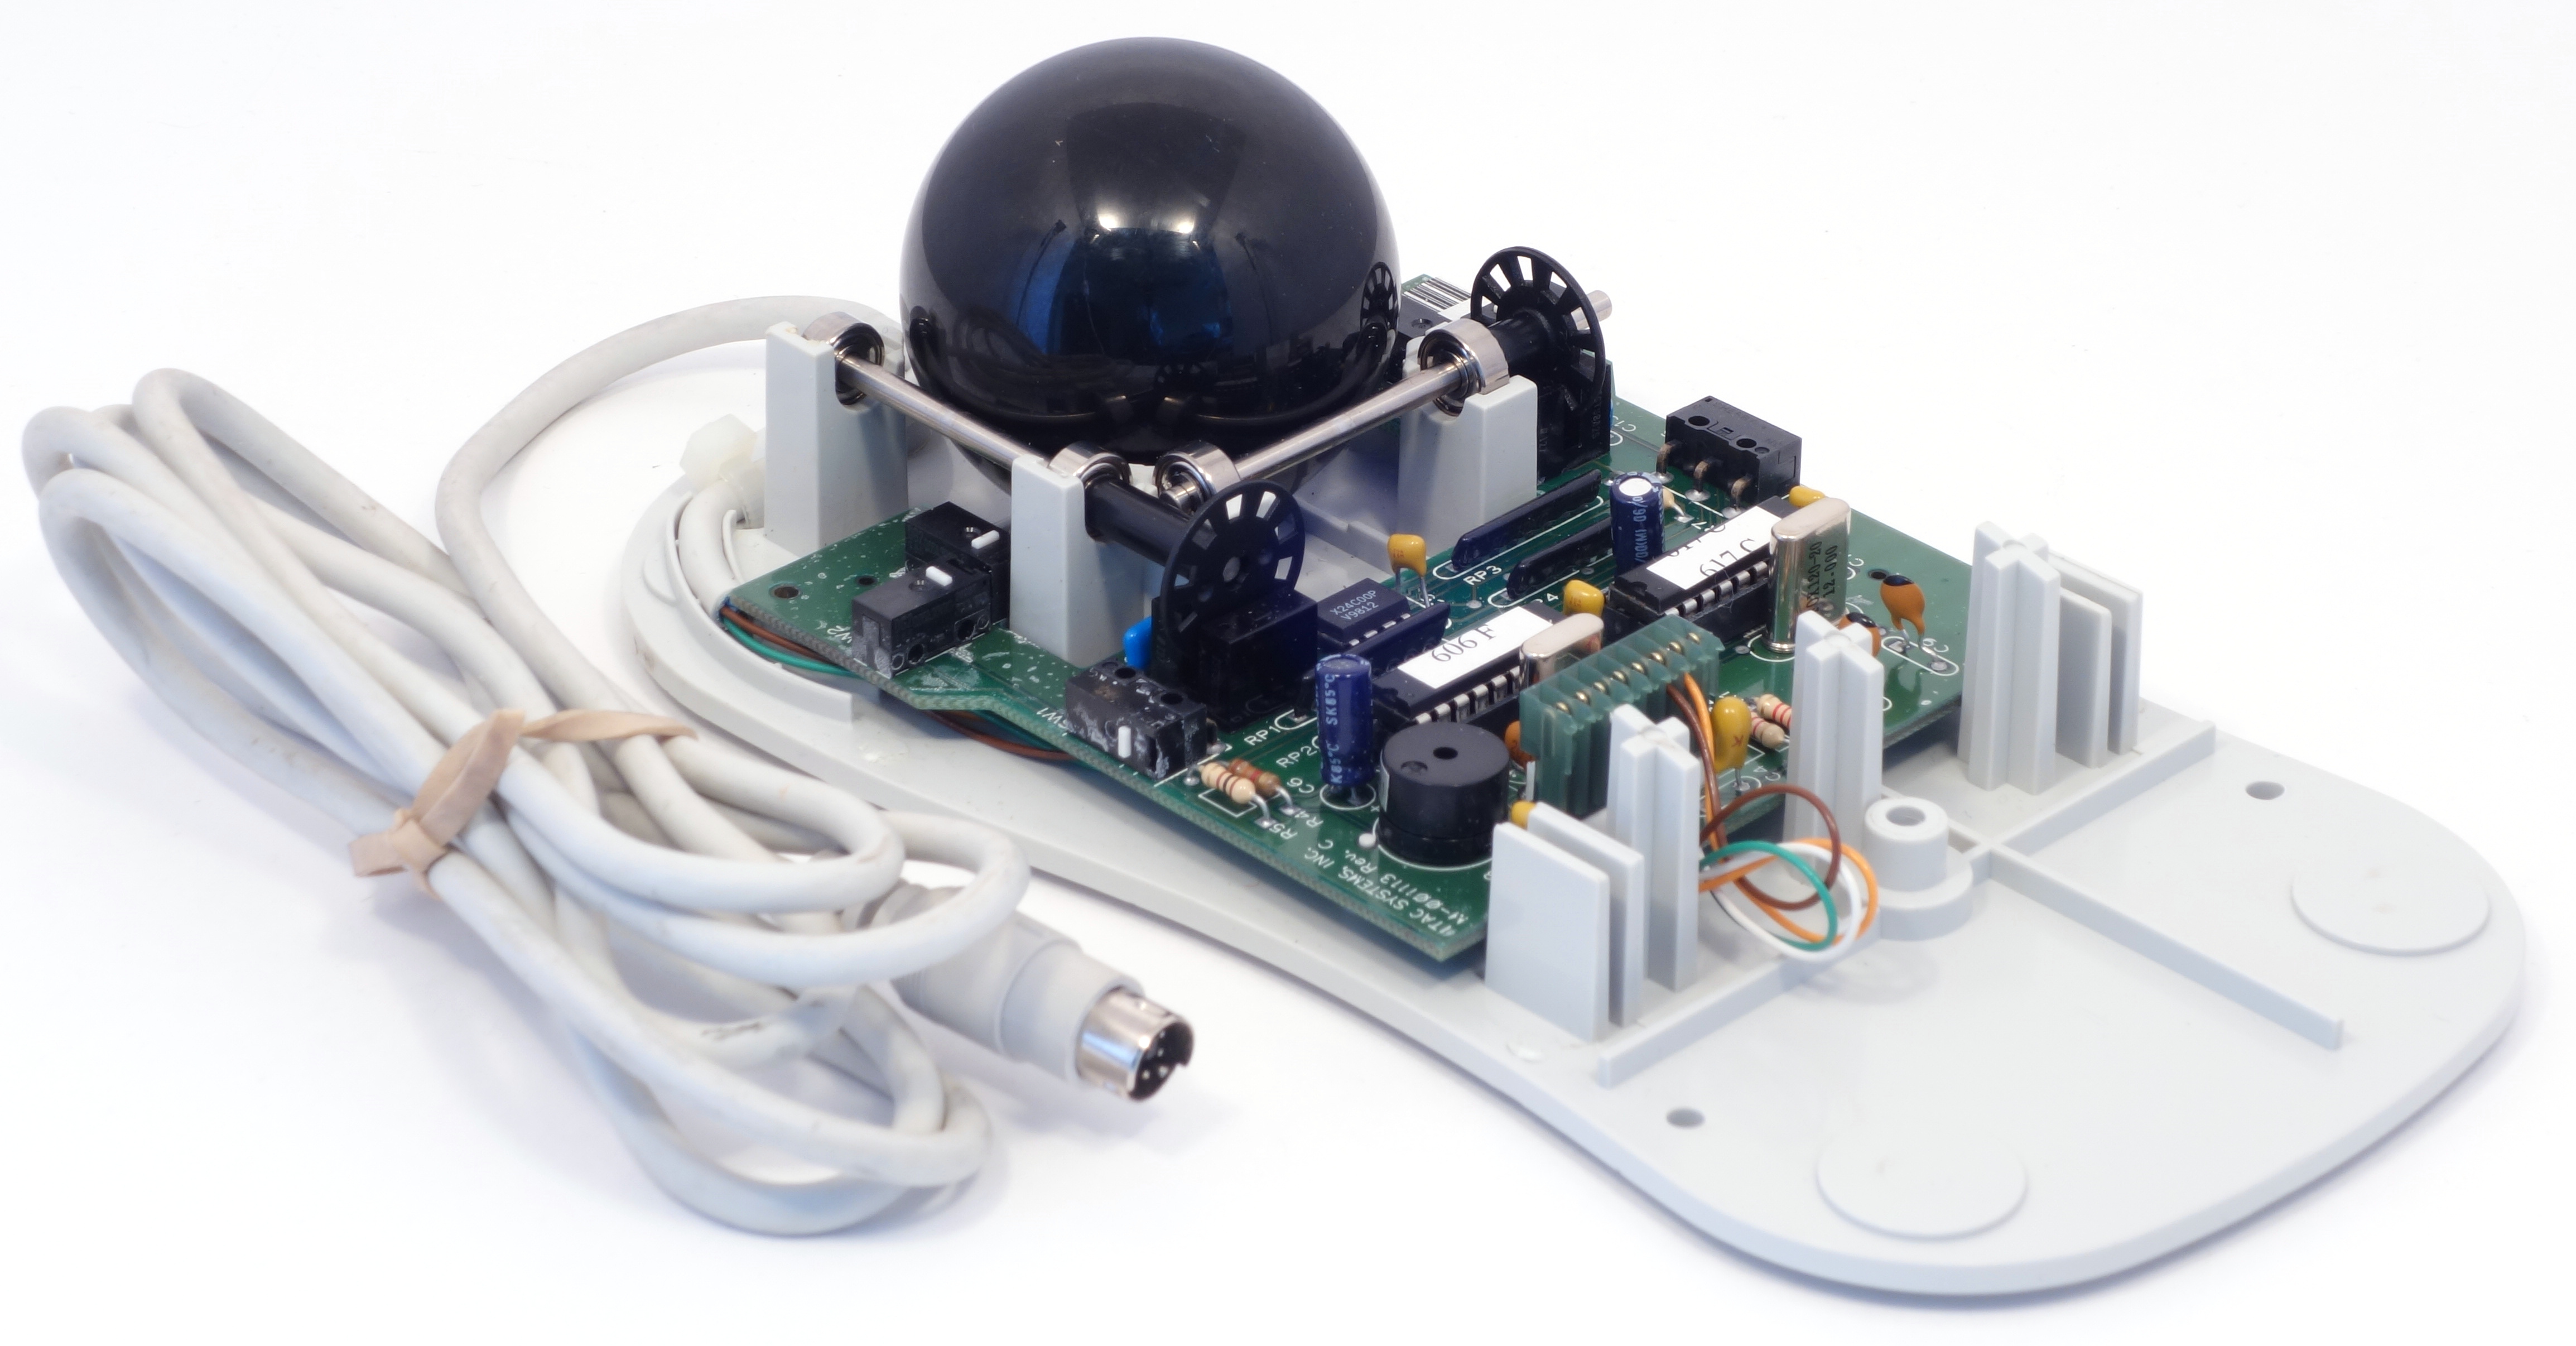
\includegraphics[scale=0.5]{1997_mousetrak_evolution/inside_30.jpg}
    \caption{evolution MOUSE-TRAK в разобранном состоянии}
    \label{fig:evolutionMOUSE-TRAKInside}
\end{figure}

\begin{thebibliography}{9}
\bibitem{announcement} ITAC Systems announces evolution MOUSE-TRAK \url{https://web.archive.org/web/19970116093947/http://www.mousetrak.com/evol.htm}
\bibitem{description} evolution MOUSE-TRAK BY ITAC \url{https://web.archive.org/web/19980116135700/http://mousetrak.com:80/index.html}
\bibitem{pcmag} M.N. Rusignuolo. Playing Cat -- and Mouse // PC MAGAZINE, October 7, 1997. -- p. 37 \url{https://books.google.by/books?id=oOfsp5YznnkC&lpg=PA37&dq=evolution%20mouse-trak&pg=PA37#v=onepage&q=evolution%20mouse-trak&f=false}
\bibitem{advanced} Evolution advanced programming procedures \url{https://web.archive.org/web/19980116134309fw_/http://mousetrak.com/evol3.htm}
\end{thebibliography}
\end{document}
